\chapter{Thiết kế giải pháp}
\section{Phương pháp kiểm tra Black Box}
Theo định nghĩa\cite{blackbox}, phương pháp black box còn được biết đến là kiểm tra hành vi, là một phương pháp kiểm thử phần mềm trong đó cấu trúc/thiết kế/hiện thực của đối tượng đang được kiểm tra không được biết đến bởi người kiểm tra.
\begin{center}
	\begin{figure}[!ht]
		\centering
		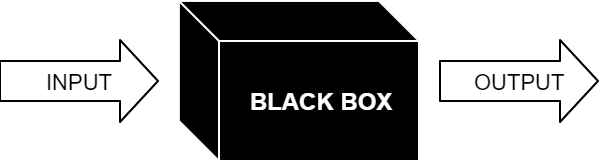
\includegraphics[width=80mm]{images/black-box.png}
		\caption{Phương pháp kiểm tra Black Box}
	\end{figure}
\end{center}
\par
Ứng dụng của chúng tôi sẽ áp dụng phương pháp kiểm tra này để đánh giá SEO cho website mà người dùng nhập vào. Cụ thể, ứng dụng sẽ tìm đến và tải về mã nguồn trang web, sau đó phân tích các thông tin nhận được, so sánh với các tiêu chí mà chúng tôi quy ước sẵn và trả về giao diện hiển thị kết quả cho người dùng.
\par
Với thiết kế này, người dùng sẽ không cần phải có kiến thức về lập trình. Ứng dụng của chúng tôi sẽ thay người dùng làm việc đó. Do đó mang lại trải nghiệm thuận tiện cho người dùng.
\par
Tuy nhiên, với giải pháp này, ứng dụng của chúng tôi sẽ xuất hiện vài khuyết điểm. Do không biết được mã nguồn chính xác của trang web, nên đôi khi trình phân tích mã nguồn của chúng tôi sẽ không ổn định, dẫn đến việc đánh giá sẽ không được chính xác hoàn toàn. Đối với các trang web được sinh ra bằng JavaScript, hiện tại thư viện phân tích mã nguồn của chúng tôi không thể tải về được cú pháp, do đó không thể kiểm tra được những trang web thuộc loại này.
\par
Nhìn chung, với việc áp dụng phương pháp kiểm tra trang web theo cơ chế black box sẽ mang đến trải nghiệm thuận tiện cho người dùng ứng dụng của chúng tôi.
\section{Kịch bản người dùng}
Chúng tôi xây dựng nên kịch bản của ứng dụng dành cho người dùng dựa trên mô hình MTV (Model - Template - View) của Django. Chúng tôi sử dụng sơ đồ bên dưới để trình bày về mô hình ứng dụng của chúng tôi.
\begin{center}
	\begin{figure}[!ht]
		\centering
		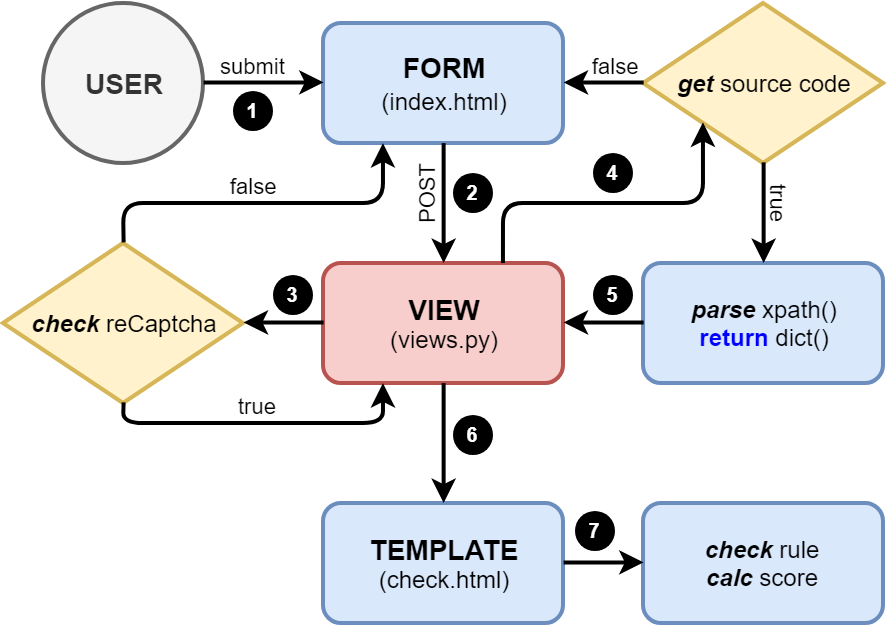
\includegraphics[width=120mm]{images/kich-ban-nguoi-dung.png}
		\caption{Kịch bản người dùng}
	\end{figure}
\end{center}
\begin{enumerate}
	\item Người dùng truy cập vào trang chủ của ứng dụng được lưu ở file \textbf{\texttt{index.html}}, tại đây hiển thị thẻ \textbf{\texttt{input}} để người dùng nhập url website cần kiểm tra.
	\item Khi người dùng bấm vào nút gửi, form sẽ gửi tín hiệu về \textbf{\texttt{VIEW}} với giao thức \textbf{\texttt{POST}}.
	\item Tại đây, chúng tôi có hàm để kiểm tra xem người dùng đã xác thực reCaptcha chưa. Nếu đúng, sẽ đi tiếp đến bước kế tiếp. Ngược lại, chúng tôi sẽ chuyển hướng người dùng về lại trang chủ và thông báo lỗi xác thực reCaptcha.
\end{enumerate}
\section{Kịch bản người dùng}
Để tạo giao diện đa nền tảng, tối ưu cho các thiết bị di động, chúng tôi sử dụng Bootstrap để quản lý tính responsive cho trang web. Ngoài ra, chúng tôi còn sử dụng thêm vài icon nữa nên sẽ lựa chọn Font Awesome vào website.
\subsection{Trang chủ}
Chúng tôi hiển thị 1 form để người dùng nhập vào URL cần kiểm tra.
\par
Để tránh kẻ xấu lợi dụng website chúng tôi để liên tục spam request đến các trang web khác. Chúng tôi sử dụng phương thức POST cho form và sử dụng thêm reCAPTCHA nhằm xác thực người dùng.
\subsection{Trang kiểm tra}
Trang này chúng tôi dùng để hiện thị thông tin được phân tích từ website của người dùng nhập vào. Kết quả sẽ được hiển thị bằng thẻ \texttt{<table>} gồm các cột:
\begin{itemize}
	\item Thành phần: Hiển thị các mục mà chúng tôi xem xét trang web người dùng, như là tiêu đề, mô tả và các thẻ khác.
	\item Trạng thái: Sử dụng icon từ Font Awesome để cho người dùng biết tiêu chí đó có đạt yêu cầu hay không. Nếu đạt yêu cầu thì sẽ hiển thị icon có dấu tích xanh lá, ngược lại trang web hiển thị dấu x đỏ kèm theo giải thích và hướng dẫn để người dùng khắc phục lỗi đó.
	\item Chi tiết: Mục này chúng tôi dùng để liệt kê ra nội dung được lấy từ trang web của người dùng, ví dụ như nội dung của thẻ tiêu đề, mô tả, hình ảnh\ldots
\end{itemize}
\par
Ngoài ra, chúng tôi sử dụng đoạn JavaScript để tính toán điểm cho website dựa trên kết quả kiểm tra, màu sắc sẽ thay đổi theo từng thang điểm:
\begin{itemize}
	\item $[80, 100]$: Màu xanh lá.
	\item $[50, 80)$: Màu vàng.
	\item $[0, 50)$: Màu đỏ.
\end{itemize}
\par
Nút Trở lại được đặt ở cuối bảng cho phép người dùng quay lại trang chủ để có thể kiểm tra trang web khác.
\subsection{Trang thông tin}
Đây là nhóm các trang web chúng tôi dùng để hiển thị đến người dùng các trang như Liên hệ, Giới thiệu.
\par
Những thủ thuật và tiêu chuẩn đánh giá của chúng tôi cũng sẽ được thêm vào nhóm này.
\section{Xử lý Backend}
Các file chúng tôi nhắc đến bên dưới nếu không có giải thích gì thêm sẽ mặc nhiên nằm trong thư mục \texttt{checkweb} mà chúng tôi đã tạo ở những phần trước.
\par
Để có thể dễ dàng quản lý các phần lập trình khi thêm vào, chúng tôi tạo thêm file \texttt{functions.py}. Tạo file \texttt{urls.py} để khai báo và quản lý các URL cho ứng dụng.
\par
Khi người dùng click vào nút submit trên trình duyệt, dữ liệu sẽ được truyền tới file \texttt{views.py} để xử lý, tại đây chúng tôi gọi đến hàm kiểm tra tính xác thực của CAPTCHA trong file \texttt{functions.py}.
\par
\texttt{views.py}
\begin{lstlisting}[language=Python]
from .functions import reCaptcha

class CheckView(TemplateView):
	def post(self, request):
		if reCaptcha(request):
			pass
			# code
\end{lstlisting}
\par
\texttt{functions.py}
\begin{lstlisting}[language=Python]
import requests
from django.conf import settings

def reCaptcha(request):
	response = request.POST["g-recaptcha-response"]
	data = {
		"secret": settings.GOOGLE_RECAPTCHA_SECRET_KEY,
		"response": response
	}
	verify = requests.post("https://www.google.com/recaptcha/api/siteverify", data=data)
	result = verify.json()
	return result["success"]
\end{lstlisting}
\par
Nếu người dùng xác thực thành công thì sẽ trả về kết quả là \texttt{True} và tiếp tục thực thi bên trong câu lệnh \texttt{if}. Tiếp theo, chúng tôi gọi hàm \texttt{parsing()} với tham số \texttt{domain} là URL website người dùng nhập vào để phân tách dữ liệu.
\par
\texttt{views.py}
\begin{lstlisting}[language=Python]
if reCaptcha(request):
	if(parsing(domain)):
		pass
		# code
\end{lstlisting}
\par
\texttt{functions.py}
\begin{lstlisting}[language=Python]
from lxml import html

def parsing(domain):
	try:
		page = requests.get(domain)
		content = html.fromstring(page.content.decode("utf-8"))
	except Exception:
		return False
		
	value = dict()
	elm = {
        "title": "//title/text()",
	}
	
	for k,v in elm.items():
		try:
			value[k] = content.xpath(v)[0]
		except Exception:
			print(k, "not found!")
			
	return value
\end{lstlisting}
\par
Đoạn code sẽ lấy ra tiêu đề của trang web và trả về kết quả vào biến \texttt{value}. Chúng tôi quay lại file \texttt{views.py} để lấy giá trị này và hiển thị ra giao diện người dùng.
\par
\texttt{views.py}
\begin{lstlisting}[language=Python]
if(parsing(domain)):
	context = parsing(domain)
	return render(request, "checkweb/check.html", context)
\end{lstlisting}
\par
Do đang sử dụng template do Django cung cấp nên file \texttt{check.html} sẽ được lưu tại \texttt{lvtn\textbackslash templates\textbackslash checkweb\textbackslash check.html}. Chúng ta có thể gọi giá trị ra giao diện bằng biến có tên là key tương ứng của biến \texttt{context}.
\par
\texttt{check.html}
\begin{lstlisting}[language=HTML]


Checking page

<!-- get variable -->
<h2>{{ title }}</h2>

\end{lstlisting}
\par
Tới đây, chúng tôi đã cung cấp những cái nhìn cơ bản cách ứng dụng của chúng tôi hoạt động. Chúng tôi sẽ tiếp tục hoàn thiện báo cáo này trong những lần cập nhật sau.